\documentclass[12pt, a4paper]{report}

% Packages :

\usepackage[french]{babel}
\usepackage[utf8]{inputenc}
\usepackage[T1]{fontenc}
\usepackage[pdftex, pdfauthor={Bacomathiques}]{hyperref}
\usepackage{sectsty}
\usepackage[explicit]{titlesec}
\usepackage{xcolor}
\usepackage{amsmath}
\usepackage{amssymb}
\usepackage{amsthm}
\usepackage{fourier}
\usepackage{titlesec}
\usepackage{fancyhdr}
\usepackage{catchfilebetweentags}
\usepackage[french, capitalise, noabbrev]{cleveref}
\usepackage[fit, breakall]{truncate}
\usepackage[margin=3cm]{geometry}
\usepackage{tocloft}
\usepackage{tikz}
\usepackage{tocloft}
\usepackage{microtype}
\usepackage{listings}
\usepackage{tabularx}
\usepackage{calc}
\usepackage[export]{adjustbox}
\usepackage[most]{tcolorbox}
\usepackage{standalone}
\usepackage{xlop}
\usepackage{etoolbox}
\usepackage{environ}

\usetikzlibrary{arrows.meta}
\usetikzlibrary{trees}

% Paramètres :

\author{Bacomathiques}
\definecolor{graphe}{HTML}{93c9ff}
\setcounter{MaxMatrixCols}{12}
\setlength{\parindent}{0pt}
\setlength{\fboxsep}{0pt}
%\pdfsuppresswarningpagegroup=1

% Code :

\lstdefinestyle{style}{
	backgroundcolor=\color{white},
	commentstyle=\em\color[HTML]{999988},
	keywordstyle=\bfseries,
	identifierstyle=\normalfont,
	stringstyle=\color[rgb]{0.87, 0.07, 0.27},
	basicstyle=\ttfamily\color{black},
	breakatwhitespace=false,
	breaklines=true,
	captionpos=b,
	keepspaces=true,
	numbers=left,
	numbersep=5pt,
	showspaces=false,
	showstringspaces=false,
	showtabs=false,
	tabsize=2,
	numbers=none
}

\lstset{style=style}
\lstset{
	literate=
	{á}{{\'a}}1
	{à}{{\`a}}1
	{ã}{{\~a}}1
	{é}{{\'e}}1
	{ê}{{\^e}}1
	{í}{{\'i}}1
	{ó}{{\'o}}1
	{õ}{{\~o}}1
	{ú}{{\'u}}1
	{ü}{{\"u}}1
	{ç}{{\c{c}}}1
}

\lstset{
	framextopmargin=10pt,
	framexrightmargin=10pt,
	framexbottommargin=10pt,
	framexleftmargin=10pt,
	xleftmargin=10pt,
	xrightmargin=10pt,
}

% Couleurs :

\definecolor{title}{HTML}{912c21}
\definecolor{section}{HTML}{1c567d}
\definecolor{subsection}{HTML}{2980b9}

\definecolor{rule}{HTML}{c4c4c4}

\definecolor{formula}{HTML}{ebf3fb}
\definecolor{formula-left}{HTML}{3583d6}

\definecolor{tip}{HTML}{dcf3d8}
\definecolor{tip-left}{HTML}{26a65b}

\definecolor{demonstration}{HTML}{fff8de}
\definecolor{demonstration-left}{HTML}{f1c40f}

\definecolor{exercise}{HTML}{e0f2f1}
\definecolor{exercise-left}{HTML}{009688}

\definecolor{correction}{HTML}{e0f7fa}
\definecolor{correction-left}{HTML}{00bcd4}

\definecolor{toc}{HTML}{fceae9}
\definecolor{toc-left}{HTML}{e74c3c}
\definecolor{toc-dark}{HTML}{87281f}

% Titres :

\renewcommand{\thesection}{\Roman{section} - }
\renewcommand{\thesubsection}{\arabic{subsection}. }

\newcommand{\sectionstyle}{\normalfont\LARGE\bfseries\color{section}}
\titleformat{\section}{\sectionstyle}{\thesection #1}{0pt}{}
\titleformat{name=\section, numberless}{\sectionstyle}{#1}{0pt}{}

\newcommand{\subsectionstyle}{\normalfont\Large\bfseries\color{subsection}}
\titleformat{\subsection}{\subsectionstyle}{\thesubsection #1}{0pt}{}
\titleformat{name=\subsection, numberless}{\subsectionstyle}{#1}{0pt}{}

\titlelabel{\thetitle\ }

% Table des matières :

\addto\captionsfrench{\renewcommand\contentsname{}}
\renewcommand{\cftsecpagefont}{\color{toc-dark}}
\renewcommand{\cftsubsecpagefont}{\color{toc-dark}}
\renewcommand{\cftsecleader}{\cftdotfill{\cftdotsep}}
\renewcommand{\cftsecfont}{\bfseries}
\renewcommand{\cftsecpagefont}{\bfseries\color{toc-dark}}
\setlength{\cftbeforetoctitleskip}{0pt}
\setlength{\cftaftertoctitleskip}{0pt}
\setlength{\cftsecindent}{0pt}
\setlength{\cftsubsecindent}{20pt}
\setlength{\cftsubsecnumwidth}{20pt}

% Commandes :

\newcommand{\newpar}{\\[\medskipamount]}
\newcommand{\lesson}[3]{%
	\newcommand{\level}{#1}%
	\newcommand{\id}{#2}%
	\hypersetup{pdftitle={#3}}
	\begin{center}%
		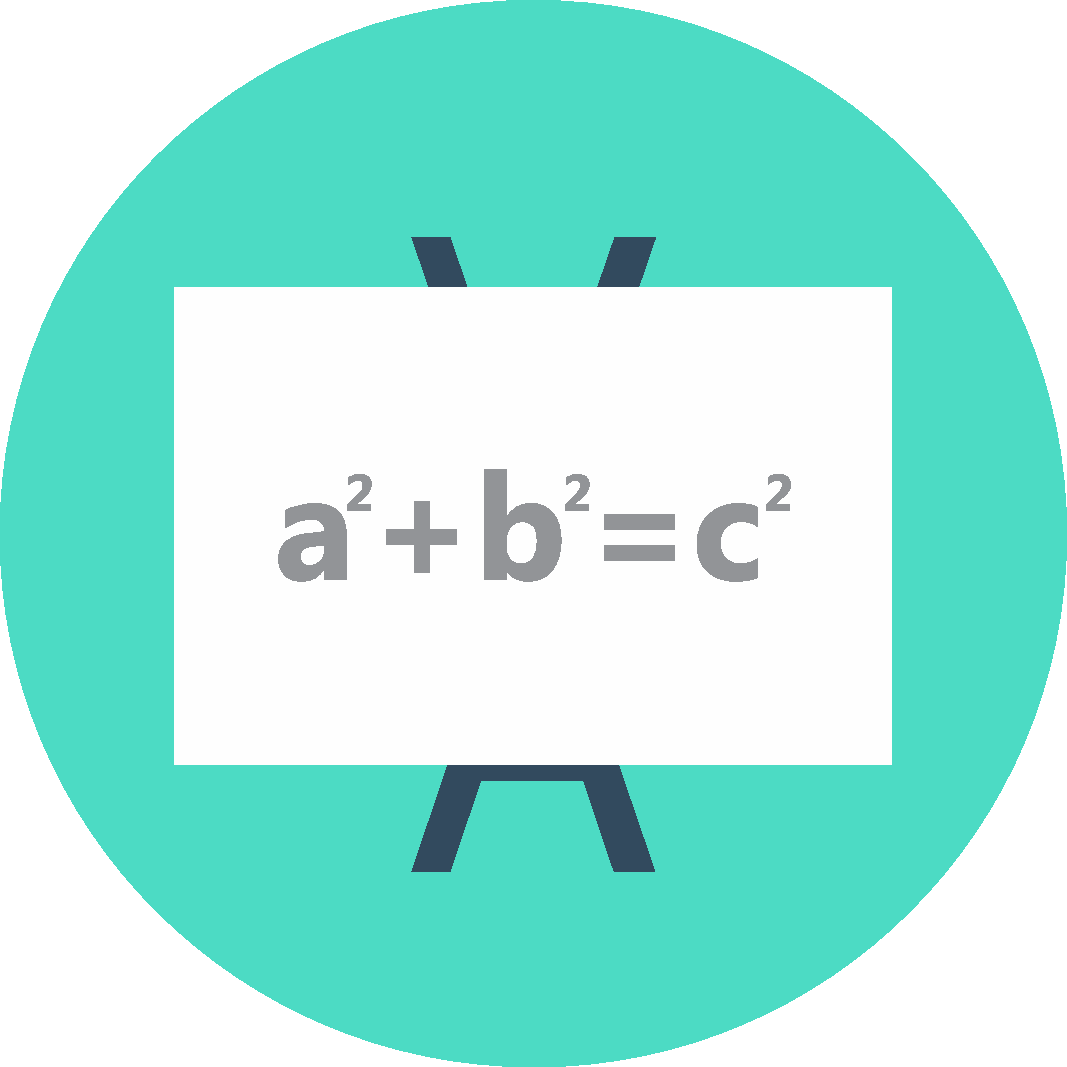
\includegraphics[width=150px]{\imagespath/bacomathiques}%
		
		\vspace{30pt}%
		{\Huge\color{title} #3}%
		
		\vspace{10pt}%
		{Bacomathiques --- \href{https://bacomathiqu.es/cours/#1/#2}{\color{section} https://bacomathiqu.es}}%
		
		\vspace{20pt}%
	\end{center}%
	\begin{toc}
		\tableofcontents%
	\end{toc}
	\thispagestyle{empty}%
	\newpage%
	\setcounter{page}{1}%
}
\newcommand{\imagespath}{../../images}
\newcommand{\lessonimagespath}{\imagespath/lessons/\level/\id/}
\newcommand{\includelatexpicture}[2][\textwidth - 100pt]{%
	\begin{center}%
		\resizebox{#1}{!}{%
			\input{\lessonimagespath#2}%
		}%
	\end{center}%
	\medskip%
}
\newcommand{\includeimage}[1]{%
	\begin{center}%
		\includegraphics{\lessonimagespath#1}%
	\end{center}%
	\medskip%
}
\newcommand{\includerepresentation}[1]{%
	\begin{center}%
		\setlength{\fboxrule}{0.5pt}%
		\href{https://www.geogebra.org/m/#1}{\includegraphics[width=\textwidth-1pt,fbox]{\lessonimagespath#1}}%
	\end{center}%
}
\newcommand{\floor}[1]{\lfloor #1 \rfloor}

\makeatletter
\newcommand\inputcontent{\@ifstar{\inputcontent@star}{\inputcontent@nostar}}
\newcommand{\inputcontent@star}[1]{%
	\ExecuteMetaData[#1]{content}%
}
\newcommand{\inputcontent@nostar}[1]{%
	\newpage%
	\inputcontent@star{#1}%
}
\makeatother

\let\oldsection\section
\renewcommand\section{\clearpage\oldsection}
\newcommand{\contentwidth}[1][medium]{}

% En-têtes :

\pagestyle{fancy}

\renewcommand{\sectionmark}[1]{\markboth{\thesection \ #1}{}}

\fancyhead[R]{\truncate{0.23\textwidth}{\color{title}\thepage}}
\fancyhead[L]{\truncate{0.73\textwidth}{\color{title}\leftmark}}
\fancyfoot[C]{\scriptsize \href{https://bacomathiqu.es/cours/\level/\id}{\texttt{bacomathiqu.es}}}

\makeatletter
\patchcmd{\f@nch@head}{\rlap}{\color{rule}\rlap}{}{}
\patchcmd{\headrule}{\hrule}{\color{rule}\hrule}{}{}
\makeatother

% Environnements :

\newenvironment{nosummary}{}{}
\newcommand{\tcolorboxtitle}[2]{\setlength{\fboxsep}{2.5pt}\hspace{-10pt}\colorbox{#1-left}{\hspace{8pt}\MakeUppercase{#2} \hspace{2pt} \includegraphics[height=0.8em]{\imagespath/bubbles/#1}\hspace{5pt}}}
\newcommand{\tcolorboxsubtitle}[2]{\ifstrempty{#2}{}{\textcolor{#1-left}{\large#2}\\[\medskipamount]}}
\tcbset{
	frame hidden,
	boxrule=0pt,
	boxsep=0pt,
	enlarge bottom by=8.5pt,
	enhanced jigsaw,
	boxed title style={sharp corners,boxrule=0pt,coltitle={white},titlerule=0pt},
	fonttitle=\fontsize{6pt}{6pt}\bfseries\boldmath,
	top=10pt,
	right=10pt,
	bottom=10pt,
	left=10pt,
	arc=0pt,
	outer arc=0pt,
}
\newtcolorbox{toc}[1][]{
	colback=toc,
	borderline west={3pt}{0pt}{toc-left},
	title=\tcolorboxtitle{toc}{Table des matières},
	colbacktitle=toc,
	before upper={\tcolorboxsubtitle{toc}{#1}}
}
\newtcolorbox{formula}[1][]{
	colback=formula,
	borderline west={3pt}{0pt}{formula-left},
	title=\tcolorboxtitle{formula}{À retenir},
	colbacktitle=formula,
	before upper={\tcolorboxsubtitle{formula}{#1}}
}
\newtcolorbox{tip}[1][]{
	colback=tip,
	borderline west={3pt}{0pt}{tip-left},
	title=\tcolorboxtitle{tip}{À lire},
	colbacktitle=tip,
	before upper={\tcolorboxsubtitle{tip}{#1}}
}
\newtcolorbox{demonstration}[1][]{
	colback=demonstration,
	borderline west={3pt}{0pt}{demonstration-left},
	title=\tcolorboxtitle{demonstration}{Démonstration},
	colbacktitle=demonstration,
	before upper={\tcolorboxsubtitle{demonstration}{#1}}
}

\NewEnviron{whitetabularx}[1]{%
	\renewcommand{\arraystretch}{2.5}
	\colorbox{white}{%
		\begin{tabularx}{\textwidth}{#1}%
			\BODY%
		\end{tabularx}%
	}%
}

% Longueurs :

\newlength{\espacetitreliste}
\setlength{\espacetitreliste}{-16pt}
\newcommand{\entretitreetliste}{\vspace{\espacetitreliste}}

\begin{document}
	%<*content>
	\lesson{terminale}{continuite-derivabilite-convexite}{Chapitre III – Continuité, dérivabilité et convexité}

	\section{Continuité}

	\subsection{Définition}

	\begin{formula}[Définition]
		Soient $f$ une fonction définie sur un intervalle $I$ et un réel $a \in I$. La fonction $f$ est continue en $a$ si on a $\lim\limits_{\substack{x \rightarrow a}} f(x) = f(a)$.
		\newpar
		$f$ est dite \textbf{continue} sur $I$, si on peut appliquer la formule ci-dessus à tous les réels de l'intervalle $I$.
	\end{formula}

	On dit de manière générale qu'une fonction est continue sur un intervalle s'il est possible de tracer sa courbe représentative sur cet intervalle ``sans lever le crayon''.

	\begin{formula}[Opérations sur les fonctions continues]
		\begin{itemize}
			\item Toute somme, produit, composée ou quotient (avec le dénominateur ne s'annulant pas) de fonctions continues est également continue sur le même intervalle.
			\item Toute fonction dérivable sur un intervalle est continue sur cet intervalle (la réciproque n'est pas vraie cependant).
		\end{itemize}
	\end{formula}

	\begin{tip}[Exemple]
		La fonction $x \mapsto \frac{1}{x}$ est continue en tout point de son ensemble de définition ($\mathbb{R}^{*}$) mais n'est pas continue sur $\mathbb{R}$.
	\end{tip}

	\subsection{Théorème des valeurs intermédiaires}

	\begin{formula}[Théorème des valeurs intermédiaires]
		Si une fonction $f$ est continue sur un intervalle $[a;b]$, alors pour tout réel $y_0$ tel que $f(a) \lt y_0 \lt f(b)$ (ou $f(a) \gt y_0 \gt f(b)$), il existe \textbf{au moins} un réel $x_0 \in [a;b]$ tel que $f(x_0) = y_0$.
	\end{formula}

	\begin{tip}[Exemple]
		Ce théorème est \textbf{très important} ! Voici un exemple : soit $f$ définie pour tout $x \in \mathbb{R}$ par $f(x) = x^3+x^2-x$. Prouvons qu'il existe au moins un réel $x_0 \in [0;3]$ tel que $f(x_0) = 5$. On a $f(0) = 0$ et $f(3) = 33$. D'après le théorème des valeurs intermédiaires, comme $f$ est continue sur $[0;3]$ et que $0 \lt 5 \lt 33$,
		il existe un réel $x_0 \in [0,3]$ tel que $f(x_0) = 5$.
		\newpar
		On peut encore tenter d'affiner la précision : $f(1) = 1$ et $f(2) = 10$. On a bien $1 \lt 5 \lt 10$ donc $x_0 \in [1;2]$, etc.
	\end{tip}

	\begin{tip}
		Une conséquence de ce théorème est que si $f(a)$ et $f(b)$ sont de signes opposés, alors la fonction $f$ s'annule au moins une fois entre $a$ et $b$.
	\end{tip}

	Enfin, il existe un corollaire qui donne en plus \textbf{l'unicité} du point $x_0$.

	\begin{formula}[Corollaire]
		Si $f$ est continue sur $[a;b]$ et que $f$ est \textbf{strictement monotone} sur cet intervalle, alors pour tout réel $y_0$ tel que $f(a) \lt y_0 \lt f(b)$ (ou $f(a) \gt y_0 \gt f(b)$), il existe \textbf{un unique} réel $x_0 \in [a;b]$ tel que $f(x_0) = y_0$.
	\end{formula}

	\subsection{La partie entière $[x]$}

	\begin{formula}[Définition]
		Soit $x \in \mathbb{R}$. La \textbf{partie entière} de $x$ notée $[x]$ (ou $E(x)$) est l'unique réel tel que : $[x] \leq x \lt [x] + 1$.
	\end{formula}

	\begin{tip}[Exemple]
		$[1,216] = 1$ et $[-2,198] = -3$.
	\end{tip}

	La fonction partie entière définie par $x \mapsto [x]$ \textbf{n'est pas continue} sur $\mathbb{R}$ :

	\includerepresentation{cpzeryjp}

	\section{Dérivation}

	\subsection{Nombre dérivé}

	\begin{formula}[Définition]
		Soient $f$ une fonction définie sur un intervalle $I$ et deux réels $a \in I$ et $h \neq 0$ tels que $(a + h) \in I$.
		\newpar
		La fonction $f$ est \textbf{dérivable} en $a$ si la limite ci-dessous existe et est finie :
		\newpar
		$\displaystyle{\lim\limits_{\substack{h \rightarrow 0}} \frac{f(a + h) - f(a)}{h}}$
		\newpar
		Ou en posant $x = a + h$ :
		\newpar
		$\displaystyle{\lim\limits_{\substack{x \rightarrow a}} \frac{f(x) - f(a)}{x-a}}$
		\newpar
		Si cette limite existe et est finie, alors elle est égale au \textbf{nombre dérivé} de $f$ en $a$, noté $f'(a)$.
	\end{formula}

	\begin{tip}[Remarque]
		Notez bien que toute fonction dérivable en un point est continue en ce point.
	\end{tip}

	\subsection{La tangente}

	\begin{formula}[Équation de la tangente]
		Soient $f$ une fonction définie sur un intervalle $I$ et un réel $a \in I$. Si $f$ est dérivable en $a$, alors la courbe représentative de $f$ admet une tangente $\mathcal{T}$ au point de coordonnées $(a; f(a))$.
		\newpar
		De plus, $f'(a)$ est le coefficient directeur de $\mathcal{T}$, et une équation de $\mathcal{T}$ est $y = f'(a)(x-a)+f(a)$.
	\end{formula}

	\begin{tip}[Exemple]
		Soit $f(x) = e^x$ définie sur $\mathbb{R}$ (voir cours sur \href{https://bacomathiqu.es/cours/premiere/fonction-exponentielle/}{la fonction exponentielle}).
		\newpar
		Cherchons une équation de la tangente au point d'abscisse $x = 0$ :
		\newpar
		On a $f'(x) = f(x)$ donc $f'(0) = 1$.
		\newpar
		Par conséquent, une équation de la tangente est $y = f'(0)(x-0)+f(0) = x + 1$ :
		on retrouve ce qui a été constaté sur \href{https://bacomathiqu.es/cours/premiere/fonction-exponentielle/#3-représentation-graphique}{la représentation graphique} de la fonction exponentielle.
	\end{tip}

	\includerepresentation{znryeret}

	\subsection{Fonction dérivée}

	\begin{formula}[Définition]
		Soit $f$ une fonction dérivable sur un intervalle $I$.
		\newpar
		On appelle fonction dérivée (ou plus simplement \textbf{dérivée}) de $f$ la fonction $g$ qui à tout réel $x$ de $I$, associe le nombre dérivé $f'(x)$ (i.e. $g(x) = f'(x)$).
	\end{formula}

	Très souvent, la fonction $g$ sera notée $f'$.

	\subsection{Applications}

	Plusieurs applications peuvent être trouvées aux dérivées. Avec le signe de la dérivée d'une fonction, il est possible d'obtenir le sens de variation de cette fonction.

	\begin{formula}[Variations d'une fonction]
		Soit une fonction $f$ dérivable sur un intervalle $I$.
		\begin{itemize}
			\item Si $f' \gt 0$ sur $I$, alors $f$ est strictement croissante sur $I$.
			\item Si $f' \lt 0$ sur $I$, alors $f$ est strictement décroissante sur $I$.
			\item Si $f' = 0$ sur $I$, alors $f$ est constante sur $I$.
		\end{itemize}
	\end{formula}

	\includerepresentation{sjeph3eh}

	Il est également possible d'en déduire diverses propriétés sur les extrema dits ``locaux'' (sur un certain intervalle) d'une fonction.

	\begin{formula}[Étude des extrema]
		Soient $f$ dérivable sur un intervalle $I$, et $a \in I$ :
		\begin{itemize}
			\item Si $f$ admet un extremum local en $a$, alors on a $f'(a) = 0$.
			\item Si $f'(a) = 0$ et que le signe de $f'$ est différent avant et après $a$, alors $f'(a)$ est un extremum local de $f$.
			\item Si $f'(a) = 0$ et qu'on est négatif avant $a$ et positif après, cet extremum local est un minimum local.
			\item Si $f'(a) = 0$ et qu'on est positif avant $a$ et négatif après, cet extremum local est un maximum local.
		\end{itemize}
	\end{formula}

	\section{Tables de dérivation}

	\subsection{Dérivées usuelles}

	Le tableau suivant est à connaître et nous donne la dérivée de la plupart des fonctions usuelles :

	\begin{formula}
		Soit $\lambda$ une constante réelle.
		\newpar
    \begin{whitetabularx}{|X|X|l|}
				\hline
				\textbf{Fonction} & \textbf{Dérivée} & \textbf{Domaine de dérivabilité} \\
				\hline
				$\lambda$ & $0$ & $\mathbb{R}$ \\
				\hline
				$x^n$ avec $n \in \mathbb{N}^*$ & $nx^{n-1}$ & $\mathbb{R}$ \\
				\hline
				\rule[-2.5ex]{0pt}{7ex}
				$\displaystyle{\frac{1}{x}}$ & $\displaystyle{-\frac{1}{x^2}}$ & $\mathbb{R}^*$ \\
				\hline
				\rule[-2.5ex]{0pt}{7ex}
				$\sqrt{x}$ & $\displaystyle{\frac{1}{2\sqrt{x}}}$ & $\mathbb{R}^+_*$ \\
				\hline
				$e^x$ & $e^x$ & $\mathbb{R}$ \\
				\hline
				\rule[-2.5ex]{0pt}{7ex}
				$\ln(x)$ & $\displaystyle{\frac{1}{x}}$ & $\mathbb{R}^+_*$ \\
				\hline
				$\sin(x)$ & $\cos(x)$ & $\mathbb{R}$ \\
				\hline
				$\cos(x)$ & $-\sin(x)$ & $\mathbb{R}$ \\
				\hline
    \end{whitetabularx}
	\end{formula}

	\subsection{Opérations sur les dérivées}

	Le tableau suivant est également à connaître et nous donne la dérivée qui dépend des opérations sur les fonctions $u$ et $v$ :

	\begin{formula}
		Soient deux fonctions $u$ et $v$ et soit $\lambda$ une constante réelle.
		\newpar
    \begin{whitetabularx}{|X|X|l|}
				\hline
				\textbf{Fonction} & \textbf{Dérivée} & \textbf{Domaine de dérivabilité} \\
				\hline
				$\lambda \times u$ & $\lambda \times u'$ & En tout point où $u$ est dérivable. \\
				\hline
				$u + v$ & $u' + v'$ & En tout point où $u$ et $v$ sont dérivables. \\
				\hline
				$u \times v$ & $u' \times v + u \times v'$ & En tout point où $u$ et $v$ sont dérivables. \\
				\hline
				\rule[-2.5ex]{0pt}{7ex}
				$\displaystyle{\frac{1}{v}}$ & $\displaystyle{-\frac{v'}{v^2}}$ & En tout point où $v$ est dérivable et non nulle. \\
				\hline
				\rule[-2.5ex]{0pt}{7ex}
				$\displaystyle{\frac{u}{v}}$ & $\frac{u' \times v - u \times v'}{v^2}$ & En tout point où $u$ et $v$ sont dérivables et non nulles. \\
				\hline
    \end{whitetabularx}
	\end{formula}

	\subsection{Dérivées de composées}

	Le tableau suivant, toujours à connaître, nous donne la dérivée des fonctions composées usuelles :

	\begin{formula}
		Soit $u$ une fonction.
		\newpar
    \begin{whitetabularx}{|X|X|l|}
				\hline
				\textbf{Fonction} & \textbf{Dérivée} & \textbf{Domaine de dérivabilité} \\
				\hline
				$u^n$ avec $n \in \mathbb{N}^*$ & $nu'u^{n-1}$ & En tout point où $u$ est dérivable. \\
				\hline
				\rule[-2.5ex]{0pt}{7ex}
				$\displaystyle{\frac{1}{u}}$ & $\displaystyle{-\frac{u'}{u^2}}$ & En tout point où $u$ est dérivable et non nulle. \\
				\hline
				\rule[-2.5ex]{0pt}{7ex}
				$\sqrt{u}$ & $\displaystyle{\frac{u'}{2\sqrt{u}}}$ & En tout point où $u$ est dérivable et strictement positive. \\
				\hline
				$e^u$ & $u'e^u$ & En tout point où $u$ est dérivable. \\
				\hline
				\rule[-2.5ex]{0pt}{7ex}
				$\ln(u)$ & $\displaystyle{\frac{u'}{u}}$ & En tout point où $u$ est dérivable et strictement positive. \\
				\hline
				$\sin(u)$ & $u'\cos(u)$ & En tout point où $u$ est dérivable. \\
				\hline
				$\cos(u)$ & $-u'\sin(u)$ & En tout point où $u$ est dérivable. \\
				\hline
    \end{whitetabularx}
	\end{formula}

	Il est cependant possible de donner une formule plus générale.

	\begin{formula}[Dérivée d'une composée]
		Soient $f$ dérivable sur $I$ et $g$ dérivable sur l'ensemble des valeurs prises par $f$ sur $I$. On a alors $(g \circ f)' = (g' \circ f) \times f'$.
	\end{formula}

	\begin{tip}[Fonction composée]
		On rappelle que la fonction $g \circ f$ est la fonction définie pour tout $x$ par $(g \circ f)(x) = g(f(x))$.
	\end{tip}

	\section{Convexité}

	\subsection{Dérivée seconde d'une fonction}

	\begin{formula}[Définition]
		Soit $f$ une fonction dérivable sur un intervalle $I$, de dérivée $f'$ dérivable sur $I$.
		\newpar
		On appelle \textbf{dérivée seconde} (notée $f''$) de $f$, la fonction dérivée de $f'$.
	\end{formula}

	Ainsi, pour calculer $f''$, on calcule d'abord $f'$, puis on dérive $f'$.

	\begin{tip}[Exemple]
		Soit $f$ la fonction définie pour tout $x \in \mathbb{R}$ par $f(x) = \sin(2x)$. Calculons $f''$.
		\newpar
		On applique la formule pour dérivée $\sin(u)$ (où $u$ est la fonction $u : x \mapsto 2x$) :
		\newpar
		Pour tout $x \in \mathbb{R}$, $f'(x) = u' \cos(u) = 2 \cos(2x)$.
		\newpar
		Pour finir, il suffit juste de dériver $f'$ : pour tout $x \in \mathbb{R}$, $f''(x) = 2 \times (-2 \sin(2x)) = -4 \sin(2x)$.
	\end{tip}

	\subsection{Fonction convexe}

	\begin{formula}[Définition]
		Soit $f$ une fonction dérivable sur un intervalle $I$, de dérivée $f'$ dérivable sur $I$.
		\begin{itemize}
			\item On dit que $f$ est \textbf{convexe} sur $I$ si $f''$ est positive sur $I$.
			\item On dit que $f$ est \textbf{concave} sur $I$ si $f''$ est négative sur $I$.
			\item On dit que $a \in I$ est un \textbf{point d'inflexion} si $f''$ change de signe en $a$ (i.e. $f''(a) = 0$ et $f''$ est positive avant $a$ puis négative après ou inversement).
		\end{itemize}
	\end{formula}

	\begin{tip}
		Dire que $f''$ est positive sur $I$ revient à dire que $f'$ est croissante sur $I$. De même, dire que $f''$ est négative sur $I$ revient à dire que $f'$ est décroissante sur $I$.
	\end{tip}

	\subsection{Lien avec les tangentes}

	\begin{formula}[Lien avec la représentation graphique]
		Soit $f$ une fonction dérivable sur un intervalle $I$, de dérivée $f'$ dérivable sur $I$. On note $\mathcal{C}_f$ la courbe représentative de $f$.
		\begin{itemize}
			\item $f$ est \textbf{convexe} sur $I$ si $\mathcal{C}_f$ est au-dessus de chacune de ses tangentes sur $I$.
			\item $f$ est \textbf{concave} sur $I$ si $\mathcal{C}_f$ est en dessous de chacune de ses tangentes sur $I$.
		\end{itemize}
	\end{formula}

	\includerepresentation{v74xn9rx}

	\begin{tip}[Exemple]
		À titre d'exemple, la fonction exponentielle est une fonction convexe.
	\end{tip}
    %</content>
\end{document}
